\chapter{Exploring new \kmer based methods for Pangenomics} %Reducing complexity of 
\label{sec:complexity}

\section{Introduction: using \kmer sets in pangenomics}%too big, too complex, too difficult to use
As discussed in the previous section of this manuscript, the  construction of pangenome as variation graphs is based on an alignment step that is well known to be accurate but computationally expensive, even if recent advances on alignment algorithms and tools, like the wavefront algorithm~\cite{wavefront} or full-text indexes like the r-index~\cite{spumoni2} and move index~\cite{movi} have provided improvement in construction time or query performance.\\
The variation graph is a feasible approach for curated analysis of a selected set of samples for large genome organisms: for example, at the time of the writing of this manuscript the Human Pangenome Reference Consortium is releasing a second batch of around 220 high quality human genomes to be used for the construction of a new reference pangenome of the Human species.\\
Finally, the alignment step implicitly requires high quality complete assemblies to produce reasonably connected graphs. While it is expected that the availability of such high quality genomes will continue growing in the coming years, there is now available a large quantity of raw (or lightly processed) data that can be used in pangenomics applications~\cite{serratus,logan} but cannot be harnessed by variation graph models.\\ 
For this reason, \kmer based approaches provide a solid alternative: as the used \kmer length is usually relatively small (from 21 to 100), they can be used also on more fragmented assemblies or directly on raw sequencing reads and their scalability is proven to be order of magnitude superior than variation graphs. Even more so: they can be used to build representations from data of different quality like phased assemblies from one cohort and unitigs from another.\\
Such tools usually use different data structures to represent internally and in an efficient way a \dbg model. The main challenge of these data structures is mainly the amount of space used to represent the \kmers versus the time used to query elements (single \kmers or sequences). For this reason, implementations decisions are often bound to optimization compromises made to achieve a specific goal: disk compression to produce small-sized indexes from large collections; fast query time of a novel sequence; time/memory trade-offs.
In any case, the computational resources to produce \ccdbg from a set of input genomes are, as shown in the previous chapter, quite lower and the tools scale to significantly larger collections.\\
As \kmer based methods present valid alternatives for pangenomic studies, I focused part of my PhD on studying and developing data structures that could find some useful application in pangenomics. Here I will present the three projects that gave birth to some relevant outcomes. On two of them, more than just working on by myself, I mostly collaborated, to different extents, with other researchers both in my unit and in other groups. While I cannot call these project as my personal contribution in the field, I believe I could bring significant input in each of them.
%As presented in the previous chapter, although using \kmer based methods for pangenomics provides the aforementioned advantages, the produced \dbg is often too big or complex to use for direct downstream applications:
%\begin{itemize}
%	\item full visualization of \dbgs for more than 10 human haplotypes is not possible with state-of-the-art computational biology tools;
%	\item when full graph visualization is possible, the repetitive regions of the genome make the graph highly connected in some parts, impeding any biological interpretation;
%	\item small region visualization is possible, usually to the scale of a gene or pseudogene, but post-processing is needed in order to polish the subgraph from parts that do not belong to the requested region, due to repetitions;
%	\item extraction of high level information is not directly possible and dependent on the construction tool: most enable presence/absence or color queries while not providing any information on where in the graph (in which unitig) the queried sequence can be found.
%\end{itemize}
%The \dbg model is therefore too complex to use for many genomic tasks, thus requiring always additional, custom scripts in order to produce information relevant for most pangenomic analyses.
The chapter will be organized as follows:
\begin{itemize}
	\item Introduction on \kmer sets and metadata representation: why it is needed and how;
	\item Overview of our contributions and my part on them;
	\item \muset: from graph to matrices for downstream analysis;
	\item Prototyping dynamic data structures for \kmer counting:
	\begin{itemize}
		\item Re-implementation of a Quotient Filter as a base for multiple applications;
		\item Explore dynamicity without indexing: super\kmer sorting;
	\end{itemize}
	\item Summary and conclusions.
\end{itemize}
%one of which is a step into providing a different representation of pangenomes as \kmer sets more suitable for downstream representation.

\section{Introduction: sets of \kmers and metadata association}
Data structures to represent a set of input genomes based on \kmers that find useful applications for pangenomics should satisfy these two main characteristics, knowing that they are, to some point, in competition:
\begin{itemize}
	\item provide efficient storage of the data;
	\item allow very fast interrogations of a \kmer or string to report the associated stored metadata;
\end{itemize}
These process to store efficiently the input data to enable fast interrogations is called indexing, while the process of the metadata interrogation is called querying. The data structures should also be able to perform this operations for large data collections, as mentioned in the introduction of this chapter. As data repository grow at a quasi-exponential trend, it has become paramount to minimize the storage requirements and query times for \kmer sets. \\
A simple but very effective analogy of indexing and querying can be done with books and words.
Let's say I remember I have a book in my library that happens to have as main character someone called Ricardo and that tells about a story that is also based in Paris. Without any organization of my library I might need to sequentially read , in the worst case, all my books from start to finish to then find the one that I was looking for. This is not convenient at all, especially if I posses a lot of books. In case I maintained an index of in which book I can find any of the words from my whole library, I could quite rapidly find the few ones that contain a character that get called Ricardito. Even more, if I had also an index that associates places with books that have scenes based in them, I could easily triangulate, without even needing to open a single book, that the one I was looking for is \emph{Travesuras de la niña mala} of the Nobel Price  Mario Vargas Llosa.
This is an example of how, indexing sequencing data, \emph{the words} and their metadata, \emph{the places}, one can rapidly check which samples, \emph{the books}, contain a requested value, without having to look at the raw data (the content of the book).\\
As the \dbg is a model for a \kmer set representation, under the hood there are different data structures that can be used to store the \kmers and index them for efficient retrieval. These data structures can be divided into exact and inexact data structures. In the rest of this section I will present the characteristics of such data structures and briefly mention some propaedeutical to the prototypes we developed.

\subsection{Hashing \kmers}
As described in section~\ref{sec:kmer}, a \kmer is a sub-string of length $k$ of a biological sequence. In order to reduce the space used to store them, the text string is converted, or hashed, into a binary string that can therefore be interpreted as an integer number. The use of the equivalence of a binary string with an integer is the basis of a great part of \kmer based data structures: from here on we will consider methods for \kmers representation as binary string using hash functions. Methods that consider \kmer as text string won't be therefore consider.
\begin{description}
	\item An hash function is any function that maps data from one set (usually text but not only) to another (usually fixed-size machine-word-length integers). The ingested value is called key and the output is usually called hash value or simply hash. They are used in a lot of applications such as a) basic computer science models like dictionaries; b) cryptography; c) bioinformatics; d) many others.
	\item hash functions should optimize on some of these properties:
	\begin{itemize}
		\item[\textbf{Uniformity}] Input data should be mapped in an uniform way in the output space: in the \kmer case, lexicographically similar \kmers should be mapped to different hashes.
		\item[\textbf{Speed}] the fastest it is possible to compute a hash from a key, the better it is. Speed depends on the number and latency of the operation executed in the computation;
		\item[\textbf{collision avoidance}] collisions, i.e. mapping different keys into the same hash, should be infrequent. The collision rate is proportional to the size of the hash space and therefore to the space that can be used to store the hash. This trade-off will be explored better in the next section.
	\end{itemize}
\end{description}
Moreover, \kmer length impacts the time/space trade-off stated in the previous section: as larger \kmer offer greater specificity, they largely increase the amount of space needed to store them (because the hash will probably be larger) as also shown for plain-text representation in section~\ref{sec:kmer}.

\subsection{Minimum set of operations and metadata}
Given a set of sequencing samples, the data structure must be able to add \kmers from each sample to itself with an \emph{insert()} operation at the moment of generation of the instance of the data structure. As will be detailed in section~\ref{sec:staticdynamic}, insertion after initial construction is not always a guaranteed feature.\\
The data structure has to be able to return the metadata associated to it, using a \memb operation. Metadata is a broad keyword that I will use to identify information associated to the \kmers represented in the data structure itself. As presence or absence of a \kmer in the set is usually directly encoded in the insertion of the elements in the data structure and do not require additional bits, data structures that report only absence or presence are considered to not support metadata. The ones that do support different kind of metadata are considered associative, i.e. associate metadata to the \kmers.\\
Finally, the data structure can conserve actively or not its internal state after a membership query. For example when looking in a dictionary if an element is present, the CPU will have inside a chunk of memory containing the queried key-value pair and other ones. Other data structures store explicit variables to remember in which place of their internal representation the \memb operation led to. This is important to notice as most of the times, sequences and not \kmers are queried to the data structure, meaning that \memb operations are done sequentially and on \kmers overlapping with each other. Leveraging these properties makes huge differences in the scalability of such data structures.

\subsubsection{Metadata types}

The most trivial case it is presence of the absence of an element inside it, using a binary \memb operation (0 for no, 1 for yes).  Other metadata that can be useful in pangenomics can be:
\begin{itemize}
	\item[\textbf{count}] If the data structure contains the number of times a \kmer has been seen in the input sample, the \memb operation will return 0 if it has never been seen, and a value $>= 1$ if the value has been seen 1 or multiple times. The count can be exact or represent an order of magnitude of the counts: this is often needed to not saturate the counts as most datasets have skewed \kmer count distribution. Counts are useful to discern copy variants number in different samples.
	\item[\textbf{colors}] In the case it remembers in which samples a \kmer has been seen, the \memb operation will return a list of containing samples for each queried \kmer. 
	\item[\textbf{Id}] In applications in which the graph structure is relevant (for example in visualization), it is useful to know in which \kmers (in the case of \dbg) or unitigs (in the case of \cdbg) of the graph it is contained the queried sequence. This case is relevant for \dbg based models.
	\item[\textbf{Text}] Text data can be used to associate \kmers to genetic information as genes, regulatory elements, flags to discern pathogenic variants from non-pathogenic ones and so on.
\end{itemize}
Of these metadata, the first two are the ones that are usually taken in consideration for query by recently developed data structures. Text data would impose a significant space requirement for the data and could be mimicked by assigning numerical labels to text and use an additional map to report the text for the \memb operation. The id information is quite overlooked by, to my knowledge, all implementations.\\
Finally, the main difference between representation of \kmer sets and sets of \kmer sets is that in the second each input sample is considered as a different set. This is done by using colors, that make possible to retrieve from the data structure in which sample a \kmer can be found.

\subsubsection{Metadata: why it is important}
Metadata is important to enable different kind of applications that need more information than just the presence or absence of a \kmer in a set. \\
In some applications it is useful to understand how many copies of a particular genetic sequence is repeated, hence its \kmer count can function as a proxy of that. The abundance of specific RNA in the cell can for example be a discriminating factor between normal and cancerous activity. The presence of a different copy number in a specific region of the DNA can discriminate between multiple phenotypes, hence highlighting differences in the samples in a pangenome: counting \kmers this is the only way to allow \dbg models to identify the multiplicity of repetitions, while in variation graphs they are implicitly encoded in the paths.\\
In some applications it is important to discern between the different samples used to fill the data structure, hence representing sets of \kmer sets. Colors are vastly used in pangenomics, as they allow to keep track of the genomes associated to variations and the ones that are part of the core genome, both in bacteria and in eukaryotes.\\
Remembering the \dbg overlap structure is also important in many applications that rely on visualization. This would enable fast subgraph identification for loci of interest and enable specific genomic applications for \dbg based methods. For example \ssh, an indexing data structure for unitigs, would be suited for this scope.\\
Finally, part or all of these these metadata might be useful to be stored at the same time for many applications, including pangenomics. For example, \kmer counts and colors are necessary at the same time to enable lossless encoding of genomes in a \dbg model (but they are not sufficient).
%The result of the \memb operation can be exact or approximate, i.e. have false positives. 

\subsection{Basic data structures: sorted list and hash table}
The most simple data structure used in computer science to maintain an ordered collection of elements to be searched in less than linear time is a sorted list of elements. By ordering the whole enumeration of the set of \kmers in each sample, one can use a binary search to find a requested \kmer in time $O$($k$log$n$), using $O$($kn$) space. This is feasible for very basic cases with small set of \kmers but it is intractable for the aforementioned use-cases, as both time to query a single element or store the dataset scale too poorly. Nevertheless, sorted list can be used in case the number of elements is greatly reduced (by using compacted \kmer representations for example) and to avoid costly indexing. More on this in section~\ref{sec:skmers}.\\
Hash-tables, a well known implementation of dictionaries (or maps) in computer science, solve the problem of the query time, bringing it to $O$($k$) or $O$(1), depending on the particular hash function used. They still require $O(kn)$ space that makes them still unusable for large collections of data. 

\subsection{Approximate membership and filters}
Approximate membership data structure offer a trade-off between the space (in memory or disk) used to store the ingested information and the probability of returning a correct answer
to improve the space efficiency. While a sorted list or a hash table return always the correct information to a query, these data structures answer with a non-zero probability of false-positive (i.e. reporting a \kmer present in the raw data when in fact it is not) and zero false-negative rates (i.e. reporting a \kmer as not present while it was present). They take the name of probabilistic data structures. Finally, the filters are data structures that resemble vectors, whose basic element (also named slots) can be single bits (hence bitvectors) or any amount of bits that ensure optimal space-efficiency and that can be smaller than a machine word or a single byte using low-level implementation operations.

\subsubsection{Bloom Filters}
Bloom filters are the most used probabilistic data structures and are used in a multitude of genomic applications, like removing from ancient DNA~\cite{akmerbroom} or non-genomic applications (non-genomic bloom filter). They are used to provide a very space-efficient representation of a set of \kmers by using a bitvector and multiple different hash functions. When an \kmer is inserted, multiple different hashes are generated and the position in the bitvector corresponding to the hashes are set to 1. When an element is queried, the same hash functions are applied and if all positions in the bitvector are set to 1 the element is considered present. If at least one position is set to 0 it means that the element is not present, thus preventing false negatives. As collision can happen, especially when using multiple hash functions, it is instead possible that a position associated to the output of a hash function of a \kmer was set to 1 by the output of another hash of another \kmer, leading to false positives, i.e. reporting a \kmer is inside the data structure while it is not present.\\
Counting bloom filters store counts instead of presence/absence in the vector positions and return an averaged value when queried.\\n which sample a 
Interleaved bloom filters instead are made by several bloom filters chunked together to report sample origin queries, when each filter si filled with \kmers from a sample.\\
Multiple implementation and optimization techniques, like the blocked-bloom filters used to speed query and insert operations, are used to maximize the potential of this data structure won't be addressed here but are thoroughly explained in these reviews~\cite{marchet2024kmersets,marchet2021kmer,marchet2024coloredkmersets}. 

\subsubsection{Quotient Filters}
Quotient filters are another data structure that is based on the idea of filling a vector with metadata but it does so in a different way compared to the bloom filter.
The hash computed from the \kmer get separated into two parts: the quotient (leftmost bits) and the remainder (the rest). The size of the quotient depends on the amount of data that is being stored. Instead of filling the vector with the metadata at the position associated to the whole hash, it fills the slot at the position associated with the quotient with the remainder. In order to avoid collision when hashes with the same quotient occur, the remainders of a quotient are stored in order in successive slots, also called runs, to preserve the information and enable fast queries. This is done by using companion data structures that are used to trace where the run of a quotient is in the vector. When metadata that is not absence or presence has to be stored, like counts, multiple slots can be used to encode the count of a single remainder, like for the Counting Quotient Filter or some bits of the slot might be reserved to store the count, like in the Backpack Quotient Filter.
These filters enable collision resolution by using slots in a more flexible way. More about this data structure will be discussed in section~\ref{sec:qf}.

\subsection{Static vs Dynamic data structures}
\label{sec:staticdynamic}
Another characteristic of data structures that represent \kmer sets is the possibility to modify the data contained in them after the initial construction. This division is therefore between what are called static and dynamic data structures. \\
A static data structure cannot be modified after construction: if a set of elements has to be added or removed from the one it was used to construct it, a new instance of the data structure has to be constructed with the modified set. These data are structure usually allow more compression of the input data, hence less space. They are suitable for applications in which a reference set is used to compare new datasets so there is no need to often modify the reference set.\\
A dynamic data structure allows a certain number of updating operations such that the input set it represents can be modified. A certain number of operations can performed, depending to the application the tool is designed for. The most common operation is the insertion of a new set of \kmers, that is equivalent to an union operation between the two sets when there is no metadata, or in the case of a counting data structure a change of the count value (if an element is already present the count is increased). Other operations can be deletion of the \kmer, or modification of the metadata associated to it. \\
While most methods are static, dynamic structures that allow efficient insertion and, less frequently, deletion of \kmers are being developed in recent years~\cite{marchet2024kmersets}.
Finally, the \kmer file format (kff) is a proposed framework that allows the lossless storing and manipulation of \kmer sets that combines space savings with interoperability across tools~\cite{kmer-file-format}.

\section{Our contributions: an outline}
The three projects span different topics and can be devised at 2 different levels of engineering. The first is mainly organizing a pipeline with some already developed bioinformatics tools and contributing to the development of a tool for \kmer information manipulation. The other two are development of a tool from scratch.\\
They can be presented as follow:
\begin{itemize}
	\item[\textbf{\muset}] is a pipeline to construct plain text unitig matrices from input sample. It enables to build an abundance matrix in which the unitig count in each sample is the average of the counts of its constituent \kmers and a presence/absence matrix that report an unitig as present in a sample if its constituent \kmers are present in the sample over a given threshold.\\
	\item[A \textbf{Quotient Filter}] implementation that, in contrast to the original one, allows dynamic updates, resizing, and a framework to develop different specific data structures on top of it. It is the building block of a novel data structure, the Backpack Quotient Filter that has been recently published. I also redeveloped a Counting Quotient filter on top of it with a \emph{Fimpera} scheme to mimic large \kmers while store smaller ones to store space.\\ 
	\item[A \textbf{Super\kmer} sorting] implementation to explore a different data structure 
\end{itemize}
Some of the research and development I did, mostly in the second and third projects just outlined, can be labeled as exploration and prototyping as the result is not intended to be a novel tool to be widely adopted by the community but as first step in possible route of research in this domain.

\section{\muset: building unitig matrices for downstream analyses}
In this section I will present the work that I have been doing on building unitig abundance matrices
\subsection{Rationale}
As presented in the introduction of this manuscript, recent advancements in genomic sequencing technologies have led to the generation of massive datasets from large-scale projects. Some of them very functional to human pangenomics such as the 1K Genomes Project and the HPRC (and many more are coming), others related to other genomic areas like transcriptomics with GEUVADIS and metagenomics with MetaSub and Tara Ocean. In pangenomics, large dataset present significant challenges for traditional variation graph analyses due to their size and complexity, as presented in the introduction of this chapter. \kmer-based methods can be instead used to study the data with techniques such as \kmer counting and matrix representation. These methods can lead to accuracy in abundance estimation of loci across multiple samples, paving the way for more comprehensive analyses of complex genomic datasets. One example is enabling GWAS studies on all possible variations inside genomes, as current ones focus only on SNPs and small indels. Another example is the possibility of use such matrices as training data for Deep Learning models to learn traits that discern healthy to non-healthy populations for specific diseases and so on.\\
For these reasons, we propose a novel method to build plain text abundance unitig matrices that can be directly used for downstream applications.

\subsection{Related work}
Cutting-edge tools that compute a \cdbg or \ccdbgs form input samples have been developed in recent years. While BCALM and Cuttlefish output   a \cdbg (hence a \kmer set) that do not record the sample of origin, \bifrost and \ggcat do build \ccdbgs that use colors to trace the source of the \kmers. While \ccdbgs are an implicit representation of an unitig matrix, as they contain the same information (unitigs and origin of \kmers) but represented in a different way, tools that build them do not produce a matrix as output nor provide any APIs or scripts to do so.\\
Recently, \kmt~\cite{kmtricks}, a very fast tool to build a \kmer abundance matrix from a set of samples has been proposed but the cardinality of the \kmer set obtained from input data renders these matrices poorly tractable for the aforementioned downstream applications. This is not a limitation of the tool but a feature of the \kmer spectrum of the datasets.\\
Remembering that unitigs, as described in section~\ref{sec:kmerobjects}, are a more succinct representation for \kmers, we propose a pipeline that mix the strength of both \cdbg tools to build unitigs and \kmt to represent \kmer color and abundance to produce unitig matrices that are more tractable for analysis. We also propose a simple pipeline to build presence absence unitig matrices from samples using a script that renders in a digestible text format the implicit representation of a \ccdbg.
\subsection{From sequencing data to unitig matrices}
The main idea behind the construction of an abundance unitig matrix is that it is now possible to construct \kmer matrices in a quite efficient way and that is is also possible to build unitigs in a quite efficient way. Therefore by compacting \kmers into unitigs and by estimating unitig abundance by averaging \kmer counts, it is possible to construct a more compact and manageable representation that preserve the high level information needed for for genomic variation diversity studies, loci variation visualization and ingestion by machine learning libraries. If abundance is not needed, presence-absence unitig matrices can still render sequence variation between individuals and be of use for diversity studies. Finally, the abundance matrix is also filtered in one of the main steps to retain only \kmers that reflect the difference between samples, while the presence-absence one does output the entire set of \kmers of the input genomes.\\
Formally, given an unitig $u$ searched in a sample $S$, the \kmer presence ratio is defined as follow:

\begin{equation}
	f(u, S) = \frac{\sum_{i=1}^{N}{x_i}}{N}
\end{equation}

while the average abundance of a unitig $u$ with respect to a sample $S$ is defined as:

\begin{equation}
	A(u, S) = \frac{\sum_{i=1}^{N}{c_i}}{N}
\end{equation}
In the equations $N$ is the number of \kmers in $u$, and $x_i$ is a binary variable that is $1$ when the $i$-th \kmer is present in sample $S$ and $0$ otherwise, while $c_i$ is a non-negative integer count.\\
Figure~\ref{fig:muset} shows the main steps of the \muset pipeline. To produce an abundance matrix, the main steps are:
\begin{enumerate}
	\item A \kmer abundance matrix is built from FASTA/FASTQ files using \kmt;
	\item \kmers that are present in at least 10\% of the samples and absent in at least 10\% of them are retained, while the others are discarded. The thresholds are customizable;
	\item Unitigs are created from this set of retained \kmers in order to compress the representation. Unitigs shorter than a certain value are discarded. While this variable can be modified by the user, our recommendation is to keep it as $2k-1$ with $k$ the length of the \kmer. This value is the minimum value to observe a SNP in the set as an unitig representing a SNP would have 2 times $k-1$ bases as overlap to the unitigs representing the adjacent bases in the genome and 1 base for the variation.
	\item The abundance unitig matrix is therefore constructed. This is done by 
	\begin{enumerate}
		\item creating a dictionary, using \ssh, to link \kmers to the unitig in which they have been compacted;
		\item each unitig abundance score is computed by summing the count of its constituent \kmer set divided by the cardinality of the set. This is done independently for each sample to retain the color information of the \kmer matrix.
	\end{enumerate} 
\end{enumerate}
To generate a presence-absence the main steps of the pipeline are:
\begin{enumerate}
	\item unitig matrix the \ccdbg is built using \ggcat. Unitigs are in FASTA format while colors are in a compress representation accessible only via \ggcat cli or APIs.
	\item unitigs are filtered by length like in step 3 of the abundance pipeline;
	\item filtered unitigs are queried against the \ggcat color index and for each sample in which at least 1 \kmer of the unitig was present, the presence ratio is reported. If no \kmer was present in the sample, the sample is not reported.
	\item the unitig query is then parsed (from jsonl) and the presence (1) or absence (0) is reported for every unitig in every sample in form of a matrix. The presence is determined when the fraction of present \kmers in the sample is above a pre-defined, although modifiable, threshold. It is also possible to produce a matrix that does report the presence ratio instead of a binary value.
\end{enumerate}
Only the abundance pipeline has been tested against the most similar state-of-the art tool that is in fact \ggcat, that produces, as mentioned, an implicit presence/absence matrix. Even without using the just presented script to produce an explicit one, the abundance matrix script is faster than \ggcat when run on a large collection of 360 ancient oral samples, as shown in table~\ref{tab:muset_comparison}. No computational resources test has been done on human genomes as it was out of the scope of the pure demonstration of the usability and efficiency of the method. 

\begin{table}[!t]
	\centering
	%\tabcolsep=2Spt
	\begin{tabular}{lccc}
		\toprule
		Method & Wall-clock time & Peak memory & Disk usage \\
		\midrule
		\muset & \textbf{9h 43m 12s} & \textbf{\SI[detect-weight=true]{19}{\textbf{\giga\byte}}} & \textbf{\SI[detect-weight=true]{1.5}{\textbf{\tera\byte}}}\\
		\ggcat & 24h 20m 40s & \SI{167}{\giga\byte} & \SI{641}{\giga\byte} \\
		\bottomrule
	\end{tabular}
	\caption{Comparison of running time, peak memory, and disk usage between \muset (filtered unitig matrix) and \ggcat (implicit and unfiltered unitigs) on 360 ancient oral samples.}\label{tab:muset_comparison}
\end{table}

\begin{figure}[h!]
	\centering
	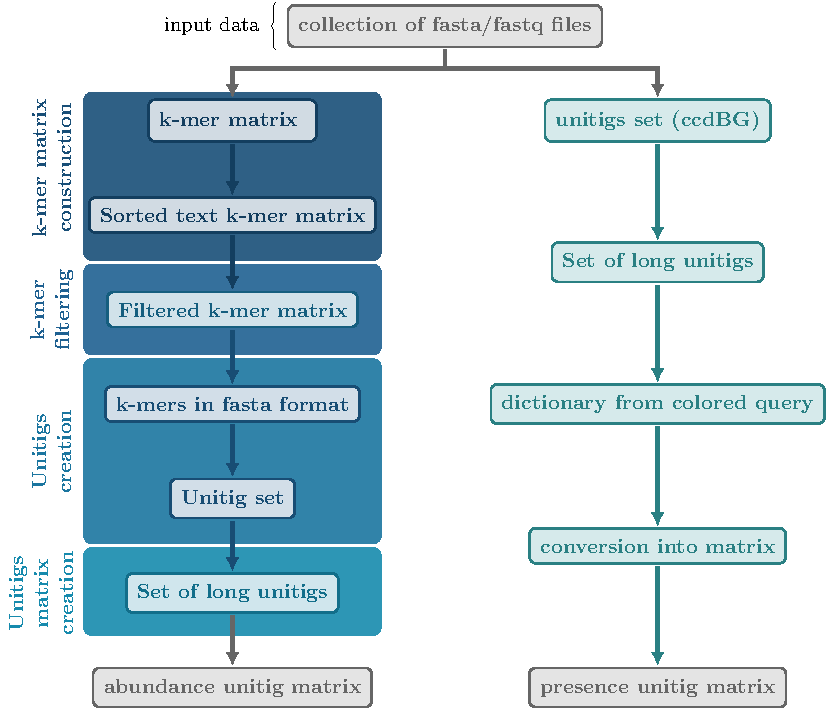
\includegraphics[width=\linewidth]{figures/kmer_methods/muset_full.pdf}
	\caption[The \muset pipeline]{Scheme representing the main steps of the \muset pipeline.}
	\label{fig:muset}
\end{figure}

\subsection{Conclusions and perspectives}
\subsubsection{Unitig matrices are pangenomes}
Although not very considered in the pangenome community, matrices are a valid pangenome representation. Every genome can be seen as a binary vector in a matrix that reports the alleles of a pangenome graph. A presence-absence matrix can be inferred by both variation graphs and \ccdbgs, in which as rows there are the ids of the nodes and as columns the input samples.  
Even if with a plain text matrix it is not possible to visualize genome variations like for graphs, they are arguably a friendlier starting point for downstream applications: biostatistics methods and population genetics can be easily generalized to this model.\\
Before \muset abundance matrices could be theoretically generated only from paths in variation graphs, while it is now possible to obtain a sufficient approximation (by averaging) for unitigs in each sample.\\
\subsection{Perspectives on other applications}
\muset is the first pipeline that uses various tools together to produce the unitig matrix representation. These tools have not been developed with this application in mind, except the \kmat software that is done to handle the various inputs and outputs format of the tools and for the filtering steps. This approach is important because it is the first to do so but it is not well optimized, as the pipeline uses various steps in which the data is dumped or read as plain text on disk, slowing the process. For this reason a future direction for this project would be to develop a tool to handle some or most of these operation in memory, gaining a lot of computing time.\\
%Another, more simple, upgrade of muset would be to produce such matrices also from a variation graph to allow 

\section{Prototyping Dynamic Data structures for \kmer counting: a Rank Select Quotient Filter}
\label{sec:qf}
While abundance unitig matrices are useful for specific genomics applications, they represent data in a way that is less efficient for others. Some use-cases require to understand if a sequence is present or absent the dataset(s) of interest in the minimum possible time. Indexing is a way to organize information in data structures that enable fast queries of the data they contain. Sequence query is done by pseudo-alignment (by \kmer~izing the sequence and query each of its \kmers). As \cdbg or \ccdbg can solve the task but the graph construction is a major bottleneck and require explicitly associating each \kmer with its abundance. \\
Approximate Membership Query (AMQ) data structures, such as Bloom filters, quotient filters, and cuckoo filters, can be used to represent a set or multi set of elements in a more efficient space. They have become essential tools not only in computational biology but also other domains like databases, storage systems and networks. Their are called approximate because they allow queries to rarely return a false positive value at a rate, $\delta$, meaning that while they will always confirm the presence of an inserted item, they might erroneously return true for non-inserted items with a probability of $\delta$. This trade-off allows the AMQ to save space. More recently, there have been developed version of these that allow to count the elements in a dataset instead of just reporting the absence or presence (cAMQ). We will focus of the ladder as they are more useful in many bioinformatics applications, from pangenomics to transcriptomics and metagenomics. For counting data structures, false positive values should report a count greater and not inferior to the real one.\\
At the present moment, the main areas of improvement of such data structures are:
\begin{enumerate}
	\item The latency of \memb operations, as it defines the kind of applications they can be used for (e.g. computer networks) and the amount of data that can be queried in a reasonable amount of time (e.g. bioinformatics). This is mostly due to a combination of the following factors:
	\begin{itemize}
		\item how well the data structure is designed in order to have data locality. Reducing cache misses by storing information such that data that might be needed consecutively fits the processor cache to save time.
		\item how well the implementation is coded, i.e. how engineered are certain operations, e.g. code branches, SIMD operations and multiprocessing. This is a very important aspect, as data structures that are less efficient in theory can in fact outperform in practice as they are easier to optimize.
	\end{itemize}
	\item The amount of space the data structure uses to store elements, that poses a hard constraint on the computer architectures that can use it. Although the cost of RAM has been declining, the amount of data is growing faster therefore pushing for more efficient use of each bit to encode information.
	\item the operation they allow, especially the possibility to modify the data structure after it has been initialized on some dataset. The most useful operations are:
	\begin{itemize}
		\item increase the count of elements, or add them if not already inside; 
		\item decrease the count of elements, or delete them if their count reaches 0;
		\item enumerate the elements inside with their respective count;
		\item automatically resize the filter when it reaches maximum capacity, to avoid the necessity to use a cardinality estimation tool a priori when initializing the data structure and allow for addition of new elements.
	\end{itemize}
\end{enumerate}
A data structure that tackles relatively efficiently all these problems has been proposed and takes the name of Counting Quotient Filter or CQF. It is based on a Rank-Select quotient filter on top of which a counting scheme has been devised in order to fill the slots of the filter with an efficient encoding of the count of the inserted element that offers less memory usage and lookup speedup compared to a Quotient Filter.

\subsection{Brief state-of-the-art overview}
The AMQ data structure that can be used in these applications are variations of three main ones: the Bloom filter, the Quotient Filter and the cuckoo filter. Although the first two have been described at the beginning of this chapter, here I briefly present them with the implementations built on top of them.
\begin{definition}
	\item[The \textbf{Bloom filter}] is a well-known AMQ, which uses hash functions to map inserted items into a bit vector. Despite its space efficiency (one to two bytes per element for common $\delta$ values like 1/50 to 1/1000), a major drawback is it cannot be resized and doesn't support deletions. Counting Bloom filters (CBF) extend Bloom filters by using saturating counters instead of bits, enabling deletions at the cost of increased space. Scalable Bloom filters, on the other hand, maintain a low false-positive rate even when the number of items is unknown by employing multiple Bloom filters.
	\item[The \textbf{Quotient filter}] uses hashed fingerprints to manage table slots. It supports a range of operations like insertion, deletion, and resizing. It is more cache-efficient and faster than Bloom filters—though less space-efficient than CBFs—making it suitable for systems like SSDs. One downside is that its performance degrades significantly once the table exceeds 60\% occupancy.
	\item[The \textbf{Cuckoo filter}] uses cuckoo hashing. It uses two potential slots for storing each item and moves items between their alternate locations if needed, causing a cascade of movements (kicks) until a stable arrangement is achieved. This filter is fast for lookups but can suffer from poor cache performance if many kicks occur, especially when the structure becomes full.
\end{definition}
About all these implementations, it is important to remember that they provide a fast lookup table in which information can be stored into fixed-size slots.\\
Finally, from now on I will discuss only about implementation details of Quotient Filter, as it is the basic data structure that we considered for out implementation. When a new element has to be inserted in a quotient filter, it is first hashed and then the resulting value is separated into a quotient of length $q$ and a remainder of length $r$.
\subsubsection{Quotient Filter structure: Rank and Select}
The Ransk-Select quotient filter, or RSQF, works by hashing items into a $p$-bit fingerprint $x$ and then dividing the bits into two parts: the quotient $h0(x)$ of $q$ bits and the remainder $h1(x)$ of $r = p - q$ bits. The RSQF has an array of $2^q$ $r$-bit slots that store the remainder of each item. When inserting an item, the filter tries to place the remainder in the slot based on the quotient. If the home slot is occupied, a linear probing technique is used to locate the next available slot.
To help tracking where the runs, i.e. the collections of subsequent slots containing the remainders of a specific quotient, are, the the RSQF uses two metadata bitvectors:
\begin{itemize}
	\item[occupieds] Tracks which slots are currently occupied by data.
	\item[runends] Indicates the end of each set of consecutive entries (or a "run") in the quotient filter.
\end{itemize}
The combination of these two bit vectors allows the RSQF to efficiently find and manage inserted items by using rank and select operations. Specifically, the \texttt{RANK} function counts the number of occupied slots up to a certain point, and  \texttt{SELECT} identifies where in the filter a particular run ends. This allows efficient lookup, insertion, and enumeration of the data in the filter.\\
Moreover, to store the data in a cache-friendly way, the filter is divided into blocks of 64 slots. To minimize operations requiring the scan of multiple blocks when the filter is relatively full, an offsets array tracks the distance from the start of a run to where it ends for every 64th slot. Therefore computing these offsets involves scanning only small sections of the metadata (64 bits or fewer) per operation, making the filter significantly faster.\\
Each block fragments both the slots vector and the metadata vectors. It contains therefore one offset value, 64 occupieds, 64 runends, and 64 slots for remainders data. By storing these elements together, the system should minimize memory access and enhances cache efficiency. 
\subsubsection{Counting}
\label{sec:rsqfcount}
Counting data structures, depending on the application, can store exact counts or order of magnitudes. This because in some applications the count number is expected relatively low and precision is important (like human genomics) while in others skewed abundance is more probable and an estimate of the count is good enough (for example in metagenomics).\\
Finally, counts can be stored with three different strategies. In any case the reminders associated to a certain quotient are stored in monotonic order inside the data structure.
\begin{enumerate}
	\item  a count can be encoded as the number of times a reminder is inserted into consecutive slots. This is the most basic implementation and the less space-efficient one as the data structure occupation would be related to the total number of counts in it. It also makes poor use of the bits in the slots that could be used for count or not.
	\item a count $N$ of a reminder $R$ can be encoded into multiple consecutive slots as follows: 
	\begin{itemize}
		\item if $1 <= N <= 2$, than the reminder $R$ is inserted $N$ times;
		\item else $K = C - 2$ can be encoded into a sequence of slots, whole boundaries are flagged by two reminders $R$ (hence the - 2). The encoding uses the slots in between to store the actual value of the count $K$. If $K$ is greater than $R$, a 0 is placed just after the first reminder to signal that the next slots are used for encoding, else not as the monotonic insertion of the reminders would implicitly flag the count. If $K$ is greater than the max value that can be encoded in the $r$ bits of a slot (i.e. $2^r -1$), it is encoded as a sum of the slots containing the count. 
	\end{itemize}
	This approach uses at least 3 slots for $n>2$ and, while more efficient than the previous one, is still quite inefficient for low count values.
	\item another way of storing $c$ is reserving $m$ extra bits for every slot to encode in it the count associated to the remainder. As this method adds $2^q * c$ bits the choice of $c$ should be calibrated for the suited application. 
\end{enumerate}

\subsection{Developing a new library for a Quotient Filter}
The implementation of the proposed CQF is efficient but represent an object that is not modifiable and does not allow for experimentation of different models based on the RSQF or CQF.
For this reason, we decided to re implement such data structure in a modular way so that the basic RSQF data structure could be used as building block for multiple applications. In this way it would be possible to develop models:
\begin{itemize}
	\item exact (when no space trade-off is chosen) or approximate;
	\item with exact or approximate counts;
	\item with different count encoding;
\end{itemize}
The developed data structure is therefore layered as this:
\begin{itemize}
	\item[\textbf{low level}] it comprises agnostic operations in the data structure such as
	\begin{itemize}
		\item setting a specific slot to a certain value. The value can be a remainder, count or combination of the two. It can also be whatever metadata as it only imposes bits to a certain region of memory corresponding to a slot;
		\item clearing of a slot to zeros for a) removals of elements from the filter and b) shifting operations;
		\item reading the value at a specific slot;
		\item shift of slots a certain amount $y$ of slots from a position $x$ of $z$ positions. This allow to keep elements when a new one has to be inserted in an already occupied position. By shifting right of $z$ slots the $y$ already set slots, the position $x$ to $x+z-1$ are therefore free to be used.
		\item metadata operation to set to 1 or to 0 the occupied and runends bits in their bitvector to keep track of which slots are in use.
		\item operation to adjourn the offset vector to keep track of the runs.
	\end{itemize}
	\item[\textbf{medium level}] it comprises operation to insert elements without explicitly caring about handling of metadata and shifts in the slots. They implement a RSQF data structure.
	\begin{itemize}
		\item addition of an element to the data structure;
		\item removal of an element from the data structure;
		\item query of an element from the data structure;
	\end{itemize}
	\item[\textbf{high level}] it comprises operations done on top of the RSQF. 
	\begin{itemize}
		\item The addition and removal are extension of the RSQF to allow for multiple operations together (i.e. adding or removing multiple slots to store the encoded counter).
		\item a function to encode and decode counters, as described in point 2 of section~\ref{sec:rsqfcount}.
		\item the query uses an intelligent linear probe that recognizes when a counter is starting and seeks the start and end of the counter of the queried reminder.
	\end{itemize}
	\item[\textbf{application specific}] application specific functions like
	\begin{itemize}
		\item hashing of \kmers
		\item initialization of the data structure
		\item enumeration of the elements inside the data structure;
		\item dynamic resize of the data structure (it comprises the enumeration of the elements, doubling the size of the filter by moving a bit from the remainder to the quotient and re-inserting all the elements);
	\end{itemize} 
\end{itemize}
This has been developed as a library or as standalone software to use.
\subsubsection{Allowing multiple types of counts: CQF and BQF}
While I focused mostly on re-implementing a CQF from the RSQF implementation, the basic implementation with low to mid level operations and application operations can be used to build other models on top of the RSQF. Victor Levallois has successfully implemented another data structure that is called the Backpack Quotient Filter (BQF), an implementation that uses the count encoding presented in point 3 of paragraph~\ref{sec:rsqfcount}.\\
This proves the flexibility of the proposed implementation.
\subsubsection{Handling toricity}
One major property of the filter that is never mentioned in the original implementation of the CQF is the handling of specific cases. Remember than runs of reminders (or counts or combination of both) associated to the same quotient are stored contiguously in a monotonic order. Moreover this has to be done in increasing slot id order. For example, when in an empty filter two elements with the same quotient are added, the slots used are the one associated with the quotient and the one \emph{on the right}, or better the one associated to the quotient+1. And so on.\\
The problem arises on the \emph{rightmost} or final part of the filter, where if new elements are added, it is probable that at some point a slot should be pushed on the next element of the final slot. To overcome this issue, the filter has a toroid structure, i.e. the next slot from the last slot is the first slot of the filter. This property avoids any problem associated with filling the filter in the final slots as it imposes a equal property to any slots of the filter.\\
Implementing the filter with such a characteristic is nontrivial as the toroid property imposes a different handling of all the comparisons inside the functions and the shifting operations.
[FIGURE HERE] 
\subsubsection{Using the Fimpera scheme to reduce space}
The size of a RSQF data structure is given by $2^q * (r + m )$ bits with $m~ 2.125$ metadata bits (and some other relatively negligible overhead). It gives that if there could be a way to store almost the same input information by reducing $r$, this would provide great space savings and allow the use of the data structure on larger datasets. To this end, bot the BQF and the CQF implementations have been developed with the Fimpera~\cite{fimpera} scheme on top.
Fimpera splits each \kmer into smaller \emph{s-mers} and stores them into the filter (each of the the \kmer count). The \kmer abundance can be therefore retrieved through its constituent \emph{s-mers} as if a \kmer is present, so are all its constituent \emph{s-mers}.\\
This approach has been demonstrated to significantly reduce the false-positive rate (by an order of magnitude) without generating false negatives or underestimating \kmer abundance~\cite{fimpera}.In this case, Fimpera is used to reduce the dimension of the filter without increasing the false-positive rate, as storing smaller hashes from \emph{s-mers} gives smaller $r$.\\
To estimate the correct abundance of a \kmer, the smallest 
The major drawback of this scheme is the loss of the \kmer enumeration feature, as only the \emph{s-mers} can be retrieved. The dynamic resizing of the data structure is instead preserved as only \emph{s-mers} are needed for that.\\
Finally, it is possible that false poisitive \kmers are introduced: \kmers that are non present in the dataset made by \emph{s-mers} that are instead found in other \kmers are going to be reported as present. As this is a joint probability, it is the result of the multiplication of each independent probability so when $s$ is large enough it is very low. This means that the $s$ parameter has to be chosen as a trade-off between space efficiency and false positive rates. For the BQF, this has been estimated as under $10^{-5}\%$ with $s > 20$ when $k = 32$. This is a reasonable false positive rate.
\subsection{Conclusions and perspectives}
This implementation could allow for other metadata to be inserted, that would render it no more a cAMQ but could for example contain color information for specific pangenomics applications. This is nontrivial as color storing is memory expensive and a new encoding would be needed. A possible lossless direction would be to use Shannon coding for the colors. If the filter is built in a way that needs multiple resizes, at each resize one could evaluate the distribution of colors and encode the most probable ones with few bits while the less recurrent ones could be encoded with less compression. \\
Finally, this implementation has not found a way as a standalone publication as the actual CQF implementation (without Fimpera) was slower than the, certainly better optimized, original one.
Nevertheless there is value in prototyping for the community data structures that are more open to customization depending on the specific application.\\
The BQF implementation has been presented at RECOMBseq~\cite{recombseq} conference and will be soon published in the associated journal~\cite{bqf}.

\section{Prototyping Dynamic Data structures for \kmer counting: Super\kmer sorted list}
\label{sec:skmers}
As seen until now in this chapter, there is no single recipe to represent \kmers in an efficient way. It depends on the specific application that is addressed. For example when comparing two different sets of datasets, one possibility is, for each set, to enumerate all the \kmers and then store them in a sorted manner in a list. The difference between the two sets will be therefore be estimated with a set metric (like the Jaccard index) that does take into account the difference between the \kmers in the two lists. This is straightforward when the two lists are sorted. Sorted lists of \kmers are also a quite fast representation for \kmer queries without indexing. Through binary search it is possible to speed the query time to $log(N)$ with N being the cardinality of the set.\\
The advantages of sorted \kmer lists are the absence of the indexation step, the predisposition for set comparison operations and the relatively fast query of the \kmer into the list. The drawback is that this representation is very expensive in terms of space. To partially overcome this issue, one can look at another side of \kmer research that is the space compression of \kmer by encoding them within a string set, i.e. all the \emph{-tigs}. The rationale is to build a set of strings in which all enumerated \kmers and nothing else can be spelled. In recent years various models have been proposed, among which unitigs, eulertigs and simplitings. Although they provide efficient storing of \kmers, sometimes together with relative biological meaning (like unitigs), they are not easy to directly query~\cite{marchet2024kmersets}.\\
Here we propose another data structure that is in between the two sides. Its aim is to:
\begin{enumerate}
	\item encode \kmers into longer strings in order to save space;
	\item maintain the sorted list structure for relative fast query of non-indexed elements.
\end{enumerate}
To do so, we build a super\kmer sorted list.\\
Super\kmers are sequences of adjacent \kmers that share the same minimizer. \\
A known uses of super\kmers is to used them in hash tables: grouping super\kmers by their minimizer enables rapid membership queries. To perform a query, one finds the set of super\kmer linked to the minimizer of the query \kmer and checks if the query \kmer appears as a sub-string within those super\kmer. Implementations like \blight~\cite{blight} and the newer \ssh~\cite{sshash}, which also has an extension that supports \kmer counts, use Minimal Perfect Hash Functions (MPHF) to facilitate mapping of minimizers to their corresponding super\kmers. The problem of using MPHF is that they generate a static dictionary that cannot be updated~\cite{smsketch}. For this reason we generate a dynamic data structure that uses sorted lists of super\kmers to store \kmer sets and, optionally, their count directly from a sequence set.
Finally, another advantage of storing super\kmers is that, since consecutive \kmers are stored together, querying sequences is quite fast, as all the ones inside the same super\kmer will be queried very fast.

\subsection{Super\kmer sorted lists: Input ad output}
The super\kmer sorting algorithm we propose is encapsulated inside a larger super\kmer data structure development I contributed to, whose details are going to be omitted for the sake of space, that already processes a set of sequences and to output an enumeration of super\kmers. Therefore the input of the algorithm is going to be a list of pre-computed super\kmers. The output is instead a list of sorted super\kmers to be used for fast lookup. While most of the operation are going to be displayed in text format, they space in which the algorithm works is binary. This is done by multiple reasons, i.e. for the parsimony of space and for fast machine operations and comparisons.

\subsection{Super\kmer list model}
In order to understand the steps of the sorting algorithm, it is helpful to imagine the super\kmer list not only as a succession of objects representing the strings but also as a matrix. The matrix is defined by 2 parameters: the number of super\kmers $N$ and the maximum length of a super\kmer $M$. $M$ is defined as $M = 2k - m$ with $k$ as the length of \kmer and $m$ as the length of the minimizer. In this model the rows are the distinct strings and the columns identify a precise position in them. As not all su per\kmers are going to be maximal,it is possible that in a certain position described by a column some super\kmer won't contain any character. This information is not explicitly encoded in the matrix but instead in the object that represent the super\kmer. Figure XXX shows the equivalences between the two models. Most of the steps of the algorithm can be considered as operations on the columns of such matrix. Another important part of this model is that at each columns position a super\kmer can have the first nucleotide of a valid \kmer or not. This depends if at that position it has a nucleotide and the next $k-1$ columns contain also valid nucleotides. If not, that column position is not valid for a \kmer. 

\subsection{Sorting \kmers in the same position}
\label{sec:skmersorting}
The fist step in the sorting algorithm requires to produce a sorted list of super\kmer ids for each column of the matrix. The sorting is done by comparing the valid \kmers at the column position using as ordering function the value of the hash of the \kmer. If the hash is smaller, it comes first.\\
To do so, a first scan over the input super\kmer is done to select the super\kmer ids of the ones that have a valid \kmer at the column position. Then, the ordering is done overt the selected list by comparing the \kmer hashes and finally the list of sorted super\kmer ids is returned. This process is done for every column of the matrix.

\subsection{Returning overlaps between \kmers}
\label{sec:skmeroverlap}
The next step is, for each pairs of consecutive columns, to detect the overlap between the $k-1$ suffix of a \kmer of the first column with the $k-1$ prefix of the subsequent. This process therefore done independently on each possible pair of consecutive columns. The $k-1$ prefixes of the \kmers of the second column are inserted in a vector. Then for each $k-1$ suffix computed from the first column, the matching value is searched in the prefix vector. If found, the pair of super\kmer ids of the first and second column is inserted in the list of candidate overlaps. Overlap is possible between a single element of one column and multiple elements of another column. In this case, all the possible overlaps are reported. At the end of the scan, each pair of column will have the list of candidate overlaps between the two.

\subsection{Maximal set of overlapping \kmers: co-linear chaining}
In the previous step all the possible \kmer overlap pairs are computed. As the ordering of the \kmers in the columns has to be respected to produce a sorted list, it naturally follows that it is possible that some overlaps won't be compatible between each other because one of the two situations occur: 
\begin{itemize}
	\item[a] the same \kmer overlaps with more than one \kmer of the the other column, but can be used just once;
	\item[b] pairs that (if visualized as edges between positions in the column) cross each other cannot be used together because they would not respect the relative order of the columns.
\end{itemize}
Figure XXX shows and example of non valid pairs and of a maximal chain while a more formal definition is provided below. To choose the maximal set of "non-crossing" pairs between the ones calculated at the previous step, we use co-linear chaining.\\
Co-linear chaining is an algorithmic technique that is known to be used in alignment algorithms. In the context of pairing elements in a sequence, it can be summarized as finding pairs of connected elements such that no "crossing" connections occur when visualized geometrically. \\
When aligning a read to a reference sequence, it takes as input pairs of maximal exact matches (MEMs). It then computes a chain of pairs such that the order of the selected pairs is concordant with the order in which they appear in the two strings while maximizing the amount of bases covered by the chain in the read. Lately it has been also used on alignment of sequences to graph in pangenomics applications.\\
\begin{definition}[Co-linear chaining of \kmers in the matrix]
	Given 
	\begin{itemize}
		\item two ordered lists of super\kmer ids of two contiguous columns computed as in section~\ref{sec:skmersorting}.
		\begin{itemize}
			\item $ A = \{a_1, a_2, ..., a_n\}, |A| = N $, representing the left column,
			\item $ B = \{b_1, b_2, ..., b_m\}, |B| = M $, representing the right column;
		\end{itemize}
		\item a set of tuples $ V = \{(v_1,w_1),(v_2,w_2), ..., (v_k,w_k) \}$ such as $ v_i \in A$ and $ w_i \in B$ and $(v_i,w_i)$ represents an overlap between \kmers of the two contiguous columns, as computed in section~\ref{sec:skmeroverlap};
	\end{itemize}
	The goal is to find the maximal list of tuples $ U$, with $set(U) \subseteq V$ such that 
	\begin{itemize}
		\item if $v_i \prec v_j$ in $U \land v_i=a_i, v_j=a_j \implies a_i \prec a_j$ in $A$, and the same for $B$;
		\item $\forall v, w \in U | v_i = a_x \lor w_i = b_y \implies \nexists v_j != v_i | v_j = a_x \land \nexists w_j != w_i | w_j = b_y$.  
	\end{itemize}
	The first condition implies that the ordering of the column lists $A, B$ is respected in $U$, while the second implies that each super\kmer id from $A$ can occur only once in the list of tuples U and the same for $B$.
\end{definition}
This problem is solved using dynamic programming~\cite{genome_scale}.\\
First the tuples in $V$ are sorted by their order in $B$. This guarantees that no "crossing" happens in the $w$ ids because $w_i = b_i: b_i \prec b_j$ will always be processed before $w_j = b_j$. To break ties on equal $v$ values, the ordering of $v_i = a_i$ in $A$ is used. Then the dynamic programming is done over the $A$ ids to find the largest set of pairs where the $A$ ids form a non-decreasing sequence. The score is therefore stored for each element $v_i$ in the list of pairs and a table $C$ of length $M$ is filled, in which index $j$ gives the maximum possible score using tuples from $V$ such that $(v,w) has w \in \{b_1,...,b_j\}$. For any tuple a recurrence is obtained depending if it violates or not the conditions above. To calculate the recurrence, 
\begin{equation} 
C[j] = \max_{j':w_{j'} \prec w_j} C[j'] + 1
\end{equation}
if  $(v_j,w_j)$ does not overlap with $ V_{j'} \subseteq \{\}(v_1,w_1),...,(v_{j-1},w_{j-1})\}$ i.e. the non-overlapping subset selected in the previous step.
To optimize the search of the best solutions $j'$ between the ones already computed, a binary search tree that contains the best score for each value $w \in A$ is queried and updated, with $O(\log{n})$ complexity. The search tree contains the $w$ values sorted by $A$ ordering. The lookup is $O(\log{n})$   From this follows that the co-linear chaining costs $O(n\log{n})$.
\subsection{Reconciliation and final output}
Once the lists of non "crossing" overlaps for each pairs have been computed using the co-linear chaining algorithm, the next step is to reconcile their information to output the sorted list. To do so, consider the matrix representation of the super\kmers, in which for each column the \kmers are sorted from top to bottom. Using the lists of non-crossing overlaps, each \kmer in the matrix is added in a map as key with value an id associated to which super\kmer it is going to be inserted. Take the case in which one of the overlap lists returns the pair (x,y) and the subsequent returns the pair (y,z). This means that \kmers x,y and z have to be compacted into the same super\kmer in the sorted list and are therefore going to be inserted in the map with the same value, e.g. 1. Other \kmers not to be compacted in the same super\kmer will have different values.\\
To output the list in an ordered way, each column of the matrix is pointed by a pointer that tracks the row in which there is the next \kmer to be inserted. A \kmer or a super\kmer is inserted in the final sorted list by iterating over the pointers. If a \kmer or super\kmer has all its elements flagged by a pointer, it is inserted in a list. Ties are broken by directly comparing the two super\kmers and inserting first the one with smallest hash. After an element is inserted, the pointers on top of its \kmers are moved to the row below. This process ir repeated until all pointer reach the last element of their column.\\

\subsection{Searching the list}
As described at the beginning of this section, the sorted super\kmer list produced by the algorithm can be used for relatively fast search without indexing the \kmers. To this end, a binary search is a fast strategy to query \kmers inside the list. Binary search is an efficient algorithm used to find the position of a target value within a sorted array. It repeatedly divides the search interval in half, comparing the middle element to the target. If the middle element matches the target, the search ends. If the target is smaller, it searches the left half, and if it's larger, it searches the right half. This process continues until the element is found or the search interval is empty.\\
When querying a \kmer in the super\kmer list, the search algorithm works as follows:
\begin{enumerate}
	\item the minimizer of the \kmers is computed and the \kmer position in a super\kmer is determined.
	\item a mask associated to that position is selected;
	\item the range of the searched list is given by $[x,y]$ and set to $[0,N]$, with $N$ being the length of the list;
	\item the binary search algorithm jumps the middle super\kmer of the range $[x,y]$;
	\item if the super\kmer does not have a \kmer at the searched position, the search moves to on to the next ones until it finds one that does;
	\item the mask is applied to the super\kmer;
	\item the resulting binary value is compared to the one of the \kmer. Here one of these 3 situations can occur:
	\begin{itemize}
		\item the masked super\kmer value is greater than the \kmer, than $[x,y]$ gets updated to $[x,y] = [(y-x/2),y]$ ;
		\item the masked super\kmer value is smaller than the \kmer, than $[x,y]$ gets updated to $[x,y] = [x,(y-x/2)]$ ;
		\item the item is found, return \texttt{FOUND} or \texttt{TRUE};
	\end{itemize}
	\item if $x = y$ return \texttt{NOT FOUND} or \texttt{FALSE}, else go back to point 4;
\end{enumerate}
The advantage of the used super\kmer representation is the search algorithm jumps an element (the super\kmer) and then looks if at a specific position, that we will call offset, there is a \kmer. By knowing the minimizer position of queried \kmer, the query can be done directly to a specific offset instead of doing a linear probe on the entire super\kmer.\\
The drawback is that, since not all super\kmers will be maximal, some queries on a specific super\kmer won't be possible, as they won't have a \kmer in the searched position. An offset will be valid if the super\kmer contains a \kmer in that position and invalid if it does not. To address this issue, when a lookup is done on a invalid offset of a super\kmer, the lookup will move as a linear probe on the previous or subsequent elements of the list until finds the first super\kmer having that offset valid.
[Could be useful to have a figure here].

%\subsection{Counting \kmers}
%As for the cqf, the super\kmer list can be also used to store \kmer counts. The storage of the count is done in another data structure like an hash table that can be used to store the average count of the \kmers in a super\kmer.
%[What more to say? And about dynamicity?]

\subsection{Conclusion and future work}
This project culminated with a prototype data structure to represent a \kmer set as a sorted list of super\kmers. The advantages of using such a representation are:
\begin{itemize}
	\item it can enumerate the \kmers in the set, differently from some hashing data structures (see bloom filters);
	\item it can compress \kmers into super\kmers thus reducing the space used to store them compared to a ordered list of \kmers;
	\item it allows fast direct queries, compared to other \emph{tigs} representations;
	\item it allows metadata to be added by a separate data structure;
\end{itemize}
This work has not been published yet but we count to close it and submit it in the coming months.

\subsubsection{Possible improvement}
As just described, the super\kmer sorted list can be queried using a variation of binary search in which, when the next super\kmer to be searched has not a valid offset, it has to linear probe the elements in the list for one that does. This slows the query operation, especially in cases where the super\kmers with a valid offset are sparse. \\
A future improvement of this algorithm would be to mitigate this issue, by adding information on non valid offsets to direct the binary search on the right direction without doing a linear probing. This strategy can be implemented by fill the bits of the super\kmer left blank when a \kmer is not stored in an informative way.\\
Given two super\kmers $S_1$ and $S_2$ in a super\kmer sorted list and an offset $t$. If there are $n$ super\kmers between $S_1$ and $S_2$ that do not have a valid \kmer at that position $t$ while $S_1$ and $S_2$ do. The strategy is to fill the bits not used by \kmers in the super\kmer with "fake" nucleotides that do not serve as genetic information but that help the search by giving information on where to find the queried \kmer. This can be done by filling the empty bits with an average between the value found in $S_1$ and $S_2$ at the same position, starting to fill the bits from the most significant one, for all $n$ super\kmers. Another approach would also take into account the cardinality $n$ of the elements to fill and, instead of filling all the super\kmers with the same averaged value, it would fill the $n$ elements with progressive values from $S_1$ to $S_2$.

\section{Does it fit to have a general conclusion of the whole chapter here?}

\printbibliography
\begin{comment}
\section{Testing the scale of humang pangenome graphs}
As a scalability and feasibility test, I built a \ccdbg using the high quality haplotypes I used for the pangenome methods evaluation proposed in the previous chapter together with the unitigs of the 1kgenomes dataset (obtained from the raw reads). This pangenome consisted of 3266 human haplotypes blended together into a single data structure (104 high quality + 3162 unitig-level assemblies). This experiment showed:
\begin{itemize}
	\item that \ccdbgs can be constructed for at least one order of magnitude more genomes than what variation graphs are now used to;
	\item that this approach could be used for several applications such as:
	\begin{itemize}
		\item structural variation inference of lower quality assemblies: even if unitigs alone cannot be used to reconstruct complex structural variations in an individual, their association in a single data structure with high quality genomes can help infer which variations are there;
		\item improvement of assembly quality by extending the unitigs of an assemblies with all the nucleotides that 
	\end{itemize}
\end{itemize}
Even if \dbg-based tools offer promising results when building pangenome graphs in terms of scalability and computational cost their use in pangenomics is still low mainly due to:
\begin{itemize}
	\item limited operations that can be performed on the data except basic \kmer interrogations on a query sequence to understand in which other genome in the model they are present;
	\item the complexity and dimension of the \ccdbgs that makes visualization and other high-level operations very difficult to be achieved.
\end{itemize}
For this reasons:
\begin{itemize}
	\item total graph visualization is not achievable for large collections (except in the case of minimizer \dbgs introduced in the previous chapter, that can give still relatively limited biological insight);
	\item large and complex regions visualization is also very difficult to achieve and gives results often confounded by repetitions, like seen in the previous chapter;
	\item downstream applications are limited by the need of in-between tools that use construction methods to achieve a representation and then use queries to infer relevant information. This is also relatively discouraged by the fact that most tools have little to no documentation and different api schemes.
\end{itemize}



\subsection{Representing sets of \kmer sets, state of the art}
\section{Indexing Data Structures}
During my thesis I focused on \kmer based algorithms, i.e. that use strings of length k as basic unit, because of their proven scalability and mathematical simplicity. Their are also the main common theoretical and technical abstraction that is used by the research group.  
Here I will briefly introduce some of the most used data structures and algorithms to store collections \kmers and, in some cases, their counts. The process to index a dataset using \kmers is to represent it as a set of the \kmers that from their sequences, like remembering the set of unique words inside one or multiple books. This representation has to be searchable so then I can interrogate it for the presence of a particular word.  There are three aspects to keep in count when considering such data structures: the computational complexity of building and, most of all, querying; the size of the data structure that stores the information and the kind of interrogations you can do with the data: presence/absence or metadata (like, for example, counts). This leads to the distinction between exact and approximate indexes and by the ones that support membership or metadata queries.\\
The membership query $memb(x)$ returns \kmers and other basic computational aspects that are at the basic of such data structure have been covered in the introduction.
\end{comment}